Considere la situación indicada en la figura, en la cual una persona arroja una pelota verticalmente hacia abajo, desde lo alto de un edificio. En el punto $A$, cuando la pelota sale de la mano de la persona, su energía potencial (respecto del suelo) es $E_{pA}$ = 8.0 J, y su energía cinética, $E_{cA}$ = 5.0 J. Despreciando la fricción con el aire durante la caída, responda:
\begin{enumerate}
    \item ¿Cuál es la energía mecánica total, $E_A$, de la pelota en $A$?
    \item ¿Cuál es la fuerza única que actúa sobre el cuerpo mientras cae? Esta fuerza, ¿es conservativa o disipativa?
    \item Entonces, ¿cuánto vale la energía mecánica $E_M$ de la pelota en $M$?, ¿y en $B$ (inmediatamente antes de tocar el suelo)?
\end{enumerate}
\begin{figure}[htb]
  \centering
  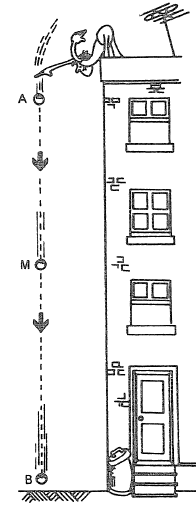
\includegraphics[scale=0.5]{enunciados/figuras/fig_alvarenga_p372_25.png}
  \caption{Alvarenga p372 Problema 25}
\end{figure}
